\chapter{Module assembly}

Usual way to assemble such kind of high-precision sensors is a manually assembly with a help of mechanical jig. Alternative way is the proposed automated assembly system.

\section{Manual assembly with mechanical jig}

One option for module assembly is manual assembly with a custom-built mechanical jig (prototype is shown on Figure \ref{fig:mechanical_jig}) \cite{Automated_assembly_slides}.

\begin{figure}[ht]\centering
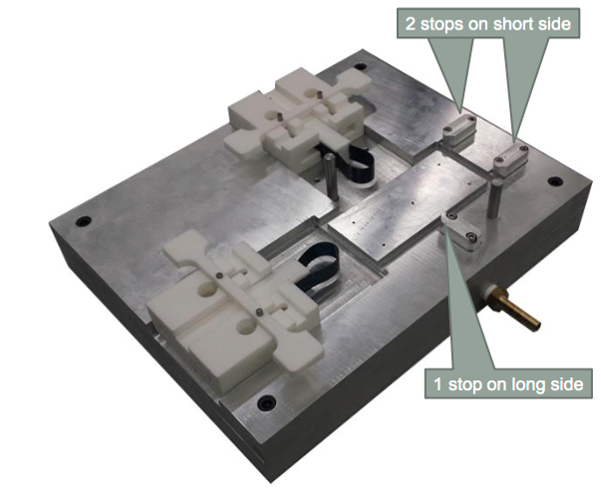
\includegraphics[width=0.7\linewidth]{Data/Module_assembly/Mechanical_jig.png}
\caption{Prototype of the mechanical jig for module assembly.}
\label{fig:mechanical_jig}
\end{figure}

With such method of assembly all parts are placed in the jig and glued together manually. To provide required accuracy mechanical jig has 3 reference stops: one along the longer side of the module and two along the shorter side. From opposite to reference stops sides the module is gently pushed by springs towards reference stops. Together they provide enough precise positioning of the module's components before and during gluing.

However such method of module assembly has a number of disadvantages. It is relatively slow and does not scale well for high number of modules to assemble. In addition, such mechanical system has poor repeatability and has no options to control the process. Moreover, it needs very precise machining technologies (several microns precision) to manufacture this mechanical jig, as well as regular calibration of reference stops positions. Finally, this mechanical system need maximum manual handling and highly depends on human operating it. This fact means that even though in theory system can provide required quality of the assembled modules, there will be always more or less several percentage of modules assembled out of required quality only because of a human mistake.

\section{Automated assembly system}

The proposed automated assembly system consists of three sub-systems: the motion subsystem, the vision subsystem and the vacuum subsystem (Figure \ref{fig:auto_assembly_system})\cite{AutomatedAssembly_tutorial}.

\begin{figure}[ht]\centering
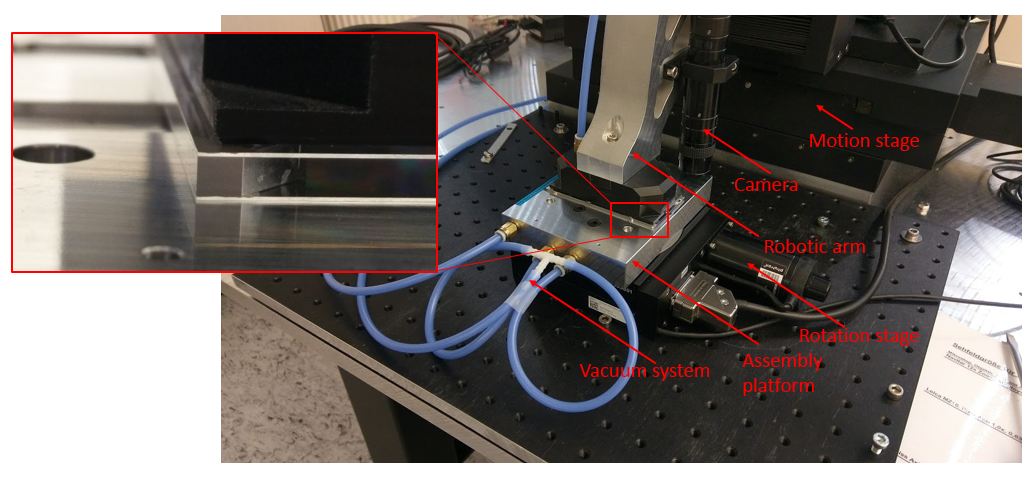
\includegraphics[width=1\linewidth]{Data/Module_assembly/Automated_assembly_system.png}
\caption{Proposed automated assembly system.}
\label{fig:auto_assembly_system}
\end{figure}

The motion system provides the precise mechanical movements needed to arrange the components comprising the SSBA. Movement of the components is achieved via mounting on the two moveable parts of the motion system: the x-y-z and rotation stages. An custom-built AL tool known as the arm is mounted on the x-y-z stage allowing mounting of components and thus movement of components in Cartesian coordinates. Components placed on the rotation stage may rotate in the horizontal plane with an angle $\theta$. The motion stages are controlled by a motion controller unit. All motion hardware is manufactured by Lang 1 with motion precisions of 4~um and 2~mrad respectively. The vacuum system enables the mounting of components to the arm and rotation stage. It consists of a single pump providing vacuum to four switchable valves which in turn distribute vacuum to independent vacuum lines. The valves are switched to on(off) states by applying a control signal of 12~(0)V. The 12V signals are provided by a relay card. One vacuum line connects to the a pickup tool which is mounted on the arm, others -- to the assembly platform. The pickup tool consists of an ESD plastic block housing an inner vacuum chamber which distributed the vacuum to an array of downward facing suction cups which slightly protrude below the bottom side of the tool. A diagram of the pickup tool is shown in Figure \ref{fig:pick_up_tool}.

\begin{figure}[ht]\centering
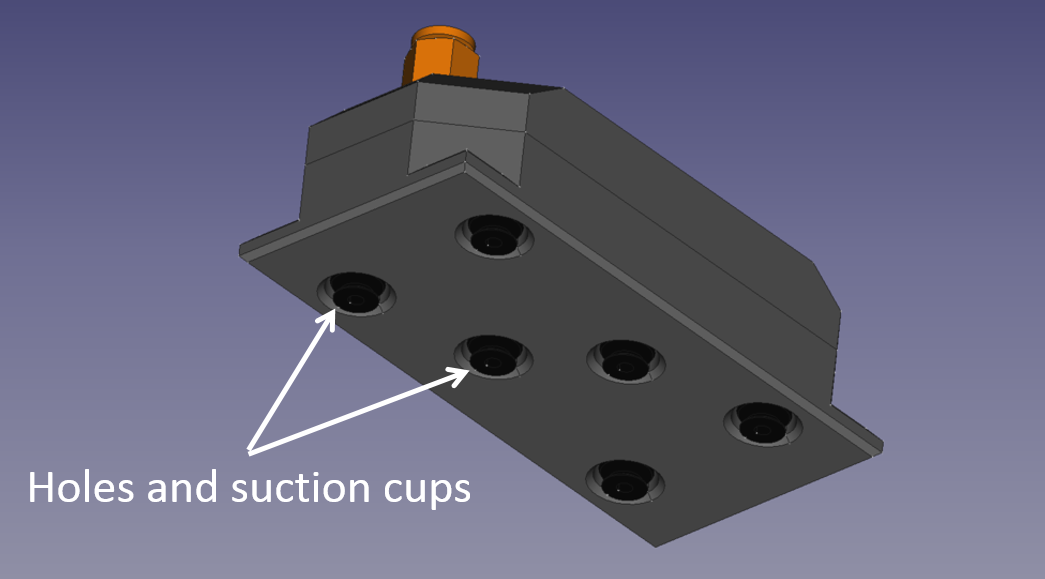
\includegraphics[width=0.7\linewidth]{Data/Module_assembly/Pick_up_tool.png}
\caption{Pick-up tool.}
\label{fig:pick_up_tool}
\end{figure}

The pickup procedure is performed by contacting the suction cups with the sensor, switching on the vacuum within the pickup tool and moving the arm directly upwards with the sensor attached. The setdown procedure is performed by contacting the mounted sensor (or baseplate) with the lower surface on which the component will be placed, switching off the vacuum in the pickup tool and moving the arm away. In order to avoid any movement of the component as the arm moves away, the component will be fixed in its setdown position with a separate array of upward-facing suction cups and independent vacuum line. The vision system acquires images of components allow determination of their positions and orientations which is crucial for precise assembly.

The vision system consists is represented by high-resolution camera by IDS. The camera is mounted on the arm and is referred to as the mobile camera. It is fixed in a downward-facing orientation. The camera acquires images immediately before pickups and immediately after setdowns in order to determine the positions of unmounted components. 

\section{Assembly platform}

One of the very important part of the automated assembly system is an assembly platform. the main purpose of it is to fix module components underneath with a vacuum.

The assembly platform should fulfil the following requirements:

\begin{enumerate}
\setlength\itemsep{-0.5em}
\item Fix all necessary module components with vacuum on top of the platform.
\item Provide the possibility of precise placement and orientation for two spacers.
\item To be reasonably light and have center of mass close to the rotation axis of a rotation stage it will be attached to.
\end{enumerate}

In order to match above mentioned requirements, the following design was proposed (Figure \ref{fig:platform_design}):

\begin{figure}[ht]\centering
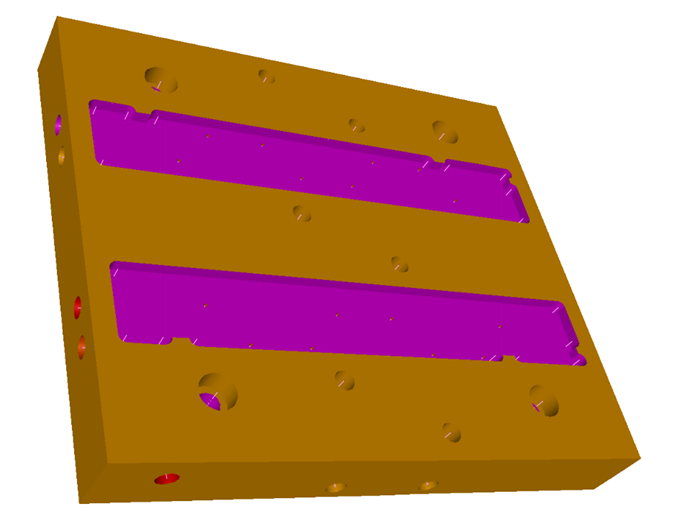
\includegraphics[width=0.7\linewidth]{Data/Module_assembly/Platform_design.png}
\caption{Design of the assembly platform.}
\label{fig:platform_design}
\end{figure}

Assembly platform has two inserts with three reference stops each to provide precise placement of spacers. Comparing to mechanical jig, assembly platform's reference stops are part of the platform itself and do not need a calibration. However having such inserts makes direct placement of the other flat components (sensors, baseplate) on top of the inserts impossible, because major area of them would have lack of underneath support under the pressure of pickup tool on top while glue curing. To solve this problem it was decided to place these components on the assembly platform perpendicular to spacers. In this case only a small area of components would have no support underneath, which is fine for assembly tasks. Perpendicular components placement on the assembly platform can be easily provided by rotation stage the platform mounted on. The platform center of mass is very close to the rotation axis (less than 1~mm) and its weight is around 1~kg thus there will no negative effects on the precision of the rotation stage operations. 

The assembly platform houses two independent inner vacuum chambers: the first for spacers holding, the second for holding other flat module components. The chamber for spacers' vacuum system distributes vacuum into the array of tiny holes (0.7~mm in diameter) on the bottom of the inserts. The size and placement of these vacuum holes is determined by the shape of spacers (Figure \ref{fig:al_spacer}). These holes do not equipped with a suction cups due to such tiny size. So small suction cups simply do not exist in the market. Additionally, the flatness of contiguous surfaces (inserts bottom and spacer) cause relatively small vacuum leakage thus providing enough tight vacuum fix of the spacers.

\begin{figure}[ht]\centering
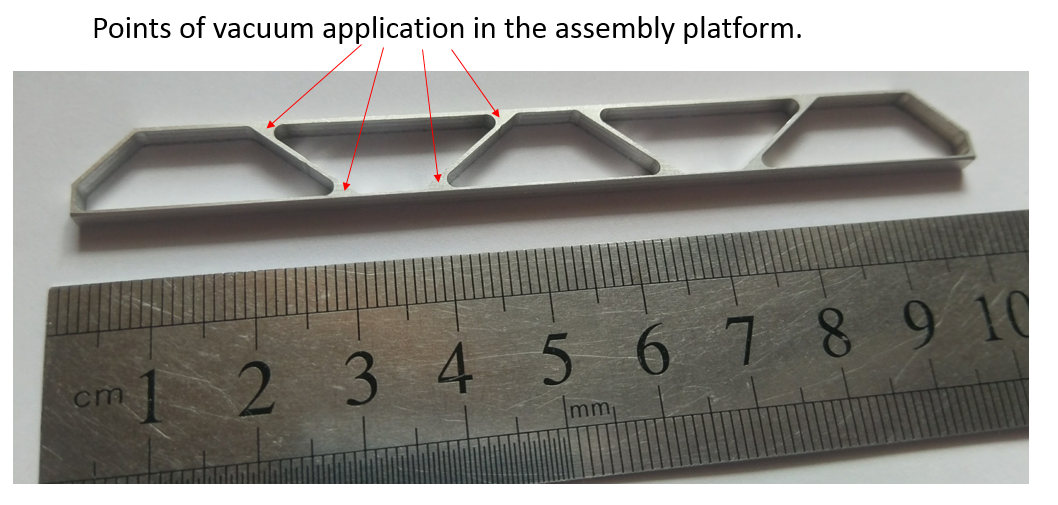
\includegraphics[width=0.7\linewidth]{Data/Module_assembly/Al_spacer.png}
\caption{Al spacer for the PS module.}
\label{fig:al_spacer}
\end{figure}

The second vacuum chamber distributes the vacuum in the array of suction cups to hold other flat module components (sensors and baseplate). It uses the same suction cups as pickup tool. Just as in the pick up tool, they stitch out a bit form the surface of the assembly platform. However, they should not prevent gluing components to spacers, stored in the inserts. That is why the depth of the interests is less than the thickness of spacers thus upper surface of the spacers stored in the inserts is a bit higher than suction cups. In other words, suction cups do not prevent operating with spacers as soon as they are lower, than upper surface of the spacers.

\section{Fast curing adhesive}

One of the crucial part of the automated assembly system is an adhesive using in the assembly, to be more  -- its curing time. Otherwise it makes a few sense to leave one module for a long time in the whole setup simply waiting the adhesive curing time. For instance, current guideline glue takes 24 hours to cure. That is why automated assembly needs a technique to avoid such long waiting. One of the proposed decision is using a small amount of fast curing adhesive in addition to main guideline glue. This adhesive should fulfil the following requirements:

\begin{enumerate}
\setlength\itemsep{-0.5em}
\item Provide reasonable bond after about 15 minutes.
\item Have no interference with main adhesive.
\item Have a thin layer (approximately less than 30~um).
\end{enumerate}

Moreover, mentioned above requirements should be completed with as small amount of fast curing adhesive as possible. For gluing tests we used simple rectangular shape Al samples (representing Al-CF spacers) and glass samples (representing Silicon sensors). Reaching listed requirements highly depends on two aspects: first -- the way fast adhesive is applied, second -- fast adhesive properties.

There are lots of possible way of applying fast adhesive: several fast adhesive drops inside main adhesive layer, several drops close to edges, bevel gluing (fill the bevel space of the Al sample with fast adhesive), side gluing (put some fast adhesive on sides), etc. For our system we decided to test bevel gluing and fast adhesive drops close to the edge. Even though bevel gluing can provide reasonable bond after 15 minutes, it is way more handy to use just two fast adhesive drops close to the edge. Adhesive was applied as shown on the Figure \ref{fig:glue_application}. 

\begin{figure}[ht]\centering
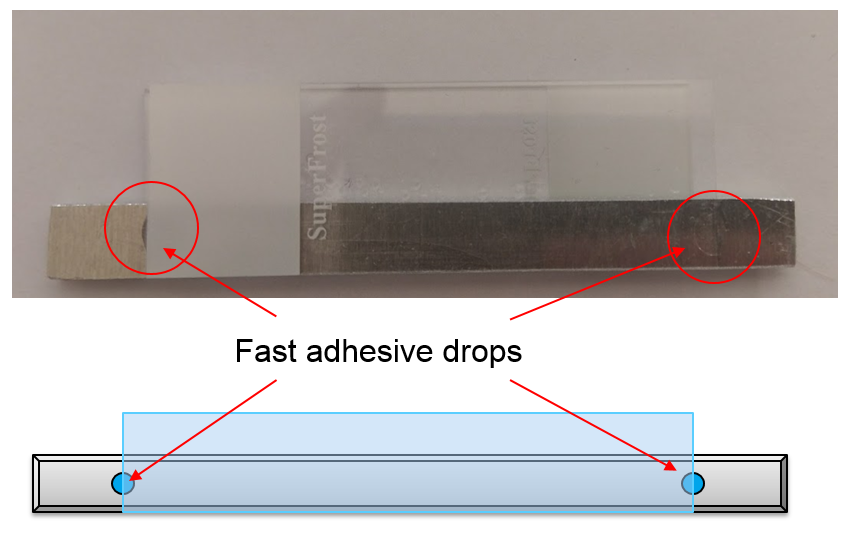
\includegraphics[width=0.7\linewidth]{Data/Module_assembly/Fast_glue_application.png}
\caption{The way of fast adhesive application during glue tests. Much smaller drops can be used for obtaining reasonable bond.}
\label{fig:glue_application}
\end{figure}

The second part of the part of the question -- finding proper fast adhesive in the market. The main issue of this question is combining two following properties: fast curing and low viscosity. Low viscosity is an integral property of the adhesive in case it should provide thin glue layer. However, fast curing means that adhesive must become hard quickly which is easier when it is initially has high viscosity. That is reason it is hard to find an adhesive combining both these properties. Nevertheless, there were several candidates for tests:

\begin{enumerate}
\setlength\itemsep{-0.5em}
\item \textit{Polytec EP 660}. According to the datasheet \cite{Polytec_EP_660_datasheet}, its curing time is about 16 hours which is too far beyond the requirements. However, the distributor said it worth trying as soon as 16 hours in a full curing time and so called handling time is shorter. Unfortunately, it this adhesive did not provide any bond after 15 minutes, as expected. The only advantage of this adhesive is that it is the same vendor as main guideline adhesive what could probably results in some financial benefits.
\item \textit{Loxeal 31-42}. According to the datasheet \cite{Loxeal_31_42_datasheet}, its full curing time is 20-30 minutes, while handling time is around 3-8 minutes. As a result it successfully provided reasonable bond after 15 minutes.
\item \textit{Wekem WK5}. According to the datasheet \cite{Wekem_WK_5_datasheet}, its curing time is around 5 minutes. It also provided reasonable bond after 15 minutes, but Loxeal adhesive has better quality and easier to operate with. Moreover, Loxeal glue provide thinner glue layer under the same pressure while curing: $<~20~um$ while Wekem provides around 40~um (Figure \ref{fig:glue_thickness}).
\end{enumerate}

\begin{figure}[ht]\centering
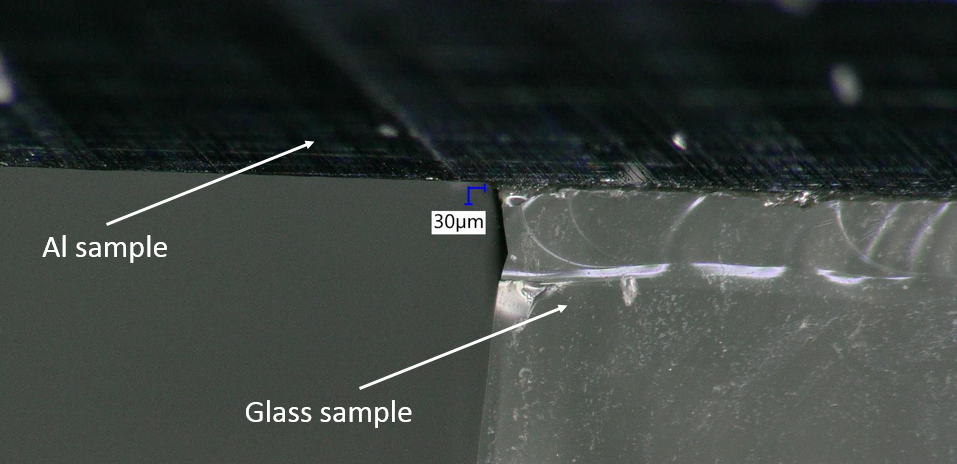
\includegraphics[width=0.7\linewidth]{Data/Module_assembly/Loxeal_393g_point_1.png}
\caption{Glue layer thickness of Loxeal~31-42 under the pressure of around $20~g/cm^{2}$}
\label{fig:glue_thickness}
\end{figure}

Talking about interaction with the main guideline adhesive, a series of test was done to check this property of the Loxeal 31-42. Among them were:

\begin{enumerate}
\setlength\itemsep{-0.5em}
\item \textit{Gluing test of two drops of fast and main adhesive in touch.} Tightness of glue bond remained approximately the same after 15 minutes curing comparing to separate fast gluing test.
\item \textit{Gluing test of two mixed drops of fast and main adhesive.} Tightness of glue bond slightly decreased after 15 minutes curing comparing to separate fast gluing test.
\end{enumerate}

To conclude, Loxeal fast adhesive clearly showed better qualities among other adhesives and fulfil all the requirements: it provides reasonable bond after 15 minutes and light pressure (around $20~g/cm^{2}$), has thin glue layer -- $<~20~um$ and show no interaction with the main guideline adhesive (touching the main adhesive).

\section{Automated assembly process}

Automated assembly process of a PS module consists of following steps:

\begin{enumerate}
\setlength\itemsep{-0.5em}
\item \emph{Prepare top sensor.} Firstly, put manually the top sensor to the platform and fix it with the vacuum. Next, detect its location and orientation with a help of camera and special software and save the data. Correct the orientation of the sensor with a help of rotation stage so thus it will be parallel to the X-axis of the motion stage. Finally, pick it up with the pickup tool and leave it attached to it. The vacuum on the pick up tool will remain applied during the whole assembly process beginning from this very first step.
\item \emph{Prepare spacers.} Once the top sensor removed from the platform and attached to the pickup tool, the platform should rotate by 90~degrees so that spacers can take their spots with the correct orientation relatively to the top sensor. Next, gently pushed to the reference stops and got fixed with the vacuum from the platform. Then the system should find and locate the reference marker on the platform thus being able to deduce the location of the spacers.
\item \emph{Glue top sensor to spacers.} Once both top sensor and spacers are ready and their locations are identified, the software can easily calculated the path for the pickup tool with attached top sensor on it. Next is to put the main adhesive and several drops of the fast adhesive on the spacers and move the pickup tool to the calculated gluing position. Special attention should be paid for Z coordinates of pickup tool moving as soon as it directly influence the thickness of the glue layer.
\item \emph{Prepare bottom sensor.} After about 15~minutes the fast adhesive drops are cured and provide reasonable bond to remove just glued spacers with top sensor. To do this pickup tool should simply move upwards with vacuum remaining applied. After the platform is cleared it should rotate by 90~degrees so that the bottom sensor can be placed and fixed with the vacuum. Next, just as for top sensor, detect its location and orientation with a help of camera and special software and save the data. Correct the orientation of the sensor with a help of rotation stage so thus it will be parallel to the X-axis of the motion stage which means parallel to the top sensor.
\item \emph{Glue bottom sensor to spacers~+~top~sensor.} All the required components for this step are fixed and theirs locations are identified. Hence the software is able to calculate the path for the pickup tool. Finally, pickup tool can move to the gluing position after applying main and fast adhesives.
\item \emph{Prepare baseplate.} After about 15-minutes glued structure can be lifted up with the pick up tool and its vacuum still remaining applied. Next is placing the baseplate paying attention for three reference pins and fix it with vacuum. These pins are not exist in the current version of the assembly platform as soon as gluing baseplate to the sensor-spacers-sensor (bare module) is not a high priority for the current state of the project. The reason for that -- baseplate gluing do not required so high accuracy as bare module.
\item \emph{Glue sensor-spacers-sensor structure (bare module) to the baseplate.} As soon as the software has already known the position of the reference marker on the assembly platform, hence it is able to calculate the location of the baseplate and the gluing position of the pickup tool with bare module attached to it. Finally, the pickup tool moves to the gluing position after applying main and fast adhesives.
\item \emph{Automated assembly is done.} After about 15 minutes fast adhesive provides enough bond and the assembled module (a part of it to be precise) can be removed from assembly platform and left for 24~hours to let the main adhesive cure. However, baseplate's reference pins fits the baseplate very tight thus manual removing can likely cause break. That is why it is better to remove the module with a pick-up tool as soon as it can provide perpendicular lift which is safer.
\end{enumerate}